Neuschnee verändert sich durch eine Schneemetamorphose. Bei der Metamorphose sublimiert Eis zu Wasserdampf und lagert sich an einer anderen Stelle wieder an. Die Geschwindigkeit dieser Umwandlung variiert je nach Umgebungsbedingungen stark. Die Temperatur im Schnee bleibt dabei relativ konstant bei 0 Grad Celsius.


Während der Metamorphose, zu sehen in Abbildung \ref{fig:Metha}, verändern sich die Eigenschaften des Schnees. Ein zentrales Prinzip dabei ist die Reduzierung der Oberfläche, was bedeutet, dass kleine Eiskristalle zu grösseren, konkaven Formen verschmelzen. Dieser Prozess ist ein Beispiel für Energieoptimierung, da das System bestrebt ist, einen energetisch günstigeren Zustand zu erreichen.

Bei der Schmelzmetamorphose bildet sich Schmelzwasser im Porenraum des Schnees. Die Umwandlung zu runden Strukturen schreitet dabei besonders schnell voran. \cite{WSLSLFMetha.2024}

Die Metamorphose, und damit die Geometrie der Eiskristalle, hat einen weitreichenden Einfluss auf den Schnee. Dies wird relevant in der Vorstudie \ref{sec:Vibr}.

\begin{figure}[H]
    \centering
    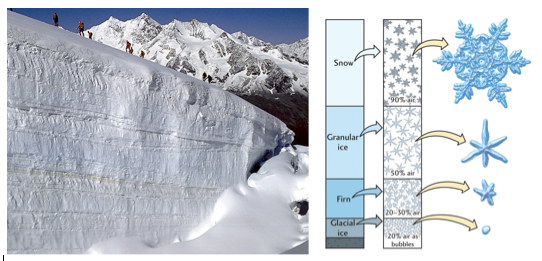
\includegraphics[width=0.9\textwidth]{Bilder/gletscher_eis_schnee.png}
    \caption{Darstellung der Schneemetamorphose, Bild aus \cite{Wetterdienst.6222017}}
    \label{fig:Metha}
\end{figure}
